La gráfica de la figura \ref{fig:carro_control} muestra la relación entre el tiempo (t) que tarda un carro de control remoto en recorrer una distancia (d) fija de 50 m y la velocidad (v) que puede tener.
\begin{minipage}[t]{0.45\linewidth}
    \begin{figure}[H]
        \centering
        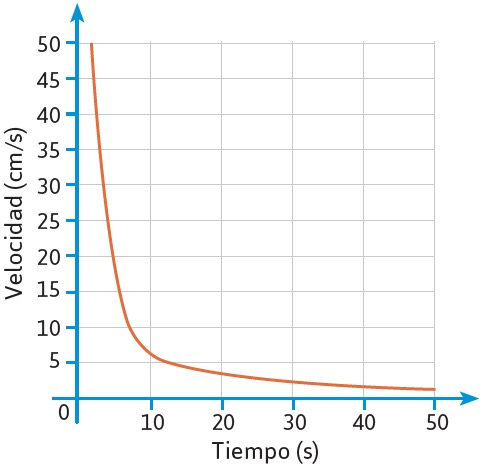
\includegraphics[width=\linewidth]{carro_control.jpg}
        \captionof{figure}{Gráfica correspondiente al movimiento del carrito de jugete.}
        \label{fig:carro_control}
    \end{figure}%
    \begin{figure}[H]
        \centering
        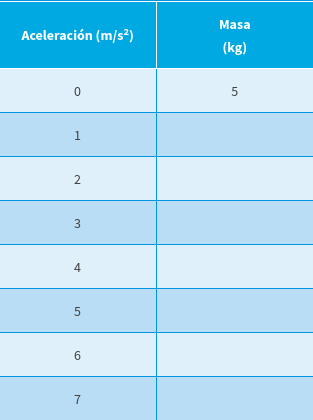
\includegraphics[width=\linewidth]{carro_control_tabla.jpg}
        \captionof{table}{Tabla correspondiente al movimiento del carrito de jugete.}
        \label{tab:carro_control_tabla}
    \end{figure}%
\end{minipage}%
\begin{minipage}[t]{0.5\linewidth}
    \begin{enumerate}
        \item De acuerdo con la gráfica, ¿cómo es la relación entre la velocidad y el tiempo? Explica.
        \item ¿Cuál es la constante de proporcionalidad para esta situación? Describe cómo la obtienen.
        \item ¿La gráfica crece o decrece? Explica.
        \item ¿En qué intervalos crece o decrece más rápido?
        \item ¿Y en cuáles crece o decrece más lento?
        \item ¿Qué sucede cuando $x$ se acerca a 0?
        \item ¿Se puede tener el caso $x = 0$? Explica.
        \item ¿Qué significa en la situación que $x=0$?
        \item ¿Qué sucede con la gráfica si los valores de $x$ aumentan?
        \item ¿Qué significa esto en la situación?
        \item Con los datos obtenidos de la gráfica, completa la tabla \ref{tab:carro_control_tabla}.
        \item ¿Qué operaciones realizan para obtener los datos de la tabla en cada caso?
        \item A partir de las operaciones que realizaron, escriban una expresión algebraica que describa la situación.
    \end{enumerate}
\end{minipage}